\chapter{Results and Discussion}
\label{chap:msms-results}

%The algorithm described in the previous chapters has been implemented in a
%in-house software called ``\ournovo'' and written in C++ language.
%It expects as input a SEQUEST-type spectrum (*.dta) which in composed by an
%header row with the precursor ion mass ($m(MH^+)$) and charge ($Q$).
%The following rows of the input spectrum file
% are composed by the peaks centroids and their intensities.
%The resulting software gives the possibility to provide a test
%sequence input, as a comparing term for the algorithm prediction, and a precursor mass, to override
%the value contained in the spectrum file.
%%to force the model to accept this value.

\section{Testing Methods}

To test the algorithm described in the previous chapters, we have applied it to a
test set kindly provided to us by \citet{fischer2005novohmm}, and originally
selected by \citet{pepnovo-analchem-2005}, of experimental mass spectra.
This test set is composed by 280 spectra of double charged peptides up to 1400 Da. coming from
tryptic spectrometry
experiments, which is accompanied by a reliable sequence assignment by SEQUEST
algorithm\cite{pepnovo-analchem-2005}. 
It originates from a 18-protein mixture database by \citet{keller2002experimental}
and from the open proteomics database by \citet{prince-2004-prot-repository}.

We compare the outcoming model prediction to the provided sequence assignment
that we refer to as ``theoretical sequence''.
To provide a measure of the prediction correctness, we compute Precision (which represents the fraction
of correctly predicted fragmentation sites over the total number of proposed
fragmentation sites),
Recall (which represents correctly predicted sites over the total number of
fragmentation sites in the theoretical sequence) and their harmonic mean,
$F$-value, for both the profile and the best sequence
as described in Sec.~\ref{sec:teo-profile}.

%This measure is calculated in two slightly different ways, considering
%two different
%definitions of \emph{correct prediction} and \emph{proposed prediction}.
%In the first way the theoretical sequence is compared to the calculated
%fragmentation
%probability accounting for matching sites weighted by their probability.
%This, in some way, compare the whole thermodynamic system, in its equilibrium
%state, to the ``real'' peptide.
%In the second way we just compare the most probable sequence, calculated as described
%in Sec.~\ref{sec:msms-issues}, to the theoretical one, without considering the
%rest of the configurations. 
%See  Sec.~\ref{sec:teo-profile} for a detailed description.

We also probe our method on a prefiltered version of test spectra, removing the
peaks that are probably noise, as explained on the following.
We also study the effect of enforcing the current parent mass, when the method
fails to identify it: as can be seen from Fig. \ref{fig:test-dm}, there is a mismatch
$\Delta m\in [-0.5,1.2]$ between the mass corresponding to the theoretical
sequence and that recovered from the .dta input file, that induced a mass error
in 47 out of 280 spectra.

\begin{figure}
\begin{center}
\resizebox{0.6\textwidth}{!}{\sffamily\input{img/msms/graph-deltamass-test}}
\end{center}
\caption{\label{fig:test-dm} Distribution of the difference between the
precursor mass reported in the .dta file and the corresponding average mass calculated
from the true sequence in the test dataset ($\Delta m$).
The figure shows that the distribution of the $\Delta m$ exit the $[-0.5,0.5]$
range where an exact estimation of the precursor mass can be done by the model.}
\end{figure}


%%%%%%%%%%%%%%%%%%%%%%%%%%%%%%%%%%%%%%%%%%%%%%%%%%%%%%%%%%%%%%%%%%%%%%%%%%%%%%%
\section{Results}

In the following we present the results of the model implementation and
testing: we divide them into results at low temperature, in which the ``best
sequence'' is  %can be 
extracted and then compared with  predictions of other \emph{de-novo} algorithms,
and results concerning the temperature dependence of some thermodynamic quantities, that 
%into temperature varying results which 
are a feature of our model and
can give an insight  of %into the thermodynamics governing the system behaviour and let the user guess 
the quality of the prediction.

\subsection{The Low-Temperature Regime: Peptide Identification}

%% Choice of the number of species used
The sequencing algorithm resulting from the system described in the previous
chapters presents two parameters still to be determined.
The first parameter is the number of ion species to use to match the
experimental peaks at each fragmentation site, while 
the second parameter is the value of the chemical potential $\mu$ introduced in
Sec.\ref{potential}.
We fix the value of those parameters to the values that optimize the predictions
of the algorithm when applied to the learning database.
%The number of ions used in the spectrum matching is, then, three in the case of
%precursors singly or doubly charged and six in the case of triply charged
%precursors.
%The coupled value of $\mu$ is then 0.48, 0.56 and 0.28 in the respective cases.

%% Choice of the working temperature
We selected as working temperature $T=1$ which was the same temperature adopted
when learning the distributions from the database.
After some
preliminary tests, we saw indeed that 
this temperature was  a good choice, as it is low enough to assure that the
system is found basically %lives 
in the energy minimum, without freezing it in the ground state or
provoking numerical problems in the computation. %singularities.}

%% Choice of the chemical potential value
At this temperature we first tested the software against a selection of
spectra from the learning database (all spectra from the database of singly
charged precursors, 1000 spectra from the doubly charged and 160 from the triply
charged)
and determined the number of ions and value of the chemical potential $\mu$ that maximizes the $F$-value
separately for each charge value.
Here $\mu$ can be interpreted as a length limiting parameter as it will
discourage configurations of the system that match many peaks just by increasing
the sequence length, using smaller residues.
Such behaviour would increase the
Recall but decrease the value of the Precision.
The resulting values for the model parameters are: for singly charged
precursors, 3 ions and $\mu(Q=1)=0.48$, for doubly charged precursors 3 ions and
$\mu(Q=2)=0.56$, and for triply charged precursors 6 ions and $\mu(Q=3)=0.28$.

We compared the results of the algorithm with other popular \emph{de novo}
sequencing algorithms, such as NovoHMM, Lutefisk, Pepnovo, Pepnovo2011 described
in the Subsec.~\ref{subsec:others}. 
They were run
with the default parameters: NovoHMM was run with the non-grouping option,
PepNovo using the CID\_IT\_TRYP model.

For every algorithm we select the most probable sequence proposed and we compare
it with the theoretical sequence provided by SEQUEST. 
To perform a model comparison we compute TP, PP and RP as well as the $F$-value
for each of the peptides.
In Table \ref{tab:tab} we report the resulting values of precision, recall and
F-value.
If precision and recall values are very close to each other,
 then the model is not generating too many
fragmentation events in order to match at least a subset (rec.$>$prec.),
neither is producing a low number of events in order not to fail
(prec.$>$rec.).
It is fair to notice that Lutefisk and PepNovo algorithms do not predict the
entire sequence if they are not sure, so that their recall
will be lower than precision, in general.


\begin{table}
\centering
\begin{tabular}{l|cccc}
\hline \hline
Model & Precision & Recall & F'-value & Mass Mismatch\\
\hline
Lutefisk       & 0.664    & 0.717    & 0.688   &43\\
PepNovo	       & 0.665    & 0.691    & 0.676   &109\\
PepNovo 2011   & 0.589    & 0.652    & 0.616   &162\\
HMM            & 0.778    & 0.786    & 0.781   &12\\
\hline
%\ournovo       & 0.611    & 0.602    & 0.605   & 47\\
%\ournovo-pre   & 0.660    & 0.638    & 0.648   & 47\\ 
%\ournovo-M     & 0.696    & 0.690    & 0.692   &  0\\
%\ournovo-pre-M & 0.754    & 0.743    & 0.749   &  0\\
\ournovo       & 0.657	  & 0.642   & 0.649   & 47\\
\ournovo-pre   & 0.663	  & 0.647   & 0.654   & 47\\ 
\ournovo-M     & 0.747	  & 0.732   & 0.739   &  0\\
\ournovo-pre-M & 0.755	  & 0.740   & 0.747   &  0\\
\hline \hline
\end{tabular}
\caption{\label{tab:tab}
In this table we report the values of Precision, Recall and $F'$-value for
different algorithms. The last column shows the number of wrongly interpreted
precursor masses. True positives are calculated as the mean of true positive
accumulated masses from N-term and from C-term, as interpretation with wrong
precursor masses can bias the result. The runs of our model have been done with
the raw algorithm (\ournovo) or over a pre-filtered spectrum (-pre) or forcing
the algorithm to accept the true precursor mass (-$M$), calculated from the
theoretical sequence.}
\end{table}

Table \ref{tab:tab} shows that the model without modifications does not present 
high precision or recall values, although, in this particular set, results are
better than PepNovo2011, while the others algorithms perform slightly better.
It is interesting to notice that the better model in this test is the one that
shows a better recognition of the peptide mass.
We have introduced some modification in order to identify the model weaknesses.
We can force the algorithm to accept an external value of the parent mass ($M$),
to enforce that the mass of the ``true'' parent sequence is considered, when
such mass is not the same as that appearing in the spectrum file. We can  also
pre-process the spectrum in order to filter out some noise peaks (-pre).
The latter filtering is performed by selecting six peaks in each window of 100 Da and
discarding the others as noise as in \citet{Mo2007}.
From the results it is clear that a higher precision in the peptide mass detection
will increase noticeably the $F'$-value, while pre-processing the spectrum
to remove the noise peaks does not  improve notably the results.

%Despite the present 
%instrument sensibility, it is usual to find erroneous values of
%the precursor mass, sometimes accountable to human data mis-interpretation.
%As shown in Fig.~\ref{fig:mh-dist}, the difference between the mass provided by
%the instrument measure of the precursor peak and reported in the spectrum file
%and the mass expected for the amino acid content of the precursor has a wide
%distribution covering a range about 6 Da, in the learning databases.
%This confuses  the interpretation process.
%Notice that the actual distribution presents some peaks uniformly separated by 1
%Da that suggests a erroneous selection of the mono-isotopic precursor peak in
%the spectrometry procedure, see Subsec.~\ref{subsec:cid-spectrum} for a detailed
%description.
%\begin{figure}
%\centering
%\subfigure[tot]{
%\includegraphics[width=2cm,angle=-90]{./img/msms/MH-dist-small-tot.eps}}
%\subfigure[$Q=1$]{
%\includegraphics[width=2cm,angle=-90]{./img/msms/MH-dist-small-q1.eps}}\\
%\subfigure[$Q=2$]{
%\includegraphics[width=2cm,angle=-90]{./img/msms/MH-dist-small-q2.eps}}
%\subfigure[$Q=3$]{
%\includegraphics[width=2cm,angle=-90]{./img/msms/MH-dist-small-q3.eps}}
%\caption{\label{fig:mh-dist}
%Precursor mass distribution as reported in the dta file of experimental data. The
%reported value is the difference in mass between the value reported in the
%experimental spectrum file and the mono-isotopic value calculated from the sequence
%proposed by SEQUEST. The Figure represent thee total distribution of the 28085
%precursor masses of the learning spectra (a), and the single distributions
%accounting for precursors with 1 (b),2 (c) or 3 (c) charges respectively.}
%\end{figure}

The same holds true in the application to the learning dataset: there
the average $F'$-value of the identification
calculated over a subset of randomly selected spectra for each
precursor fragment charge, takes lower  values: 0.565, 0.639 and 0.412
for the precursor charge state $Q=1,2,3$ respectively.
This value increases if the exact mass of the precursor peptide is passed
to the algorithm, giving 0.569, 0.659 and 0.444 respectively.
%Notice that the fraction of peptides for which the algorithm misinterprets the
%precursor mass is really high: 0.614, 0.709 and 0.613 respectively.
%As a term of comparison we applied the NovoHMM algorithm to the same spectra
%sets where we found a sensible drop in precision: $F$-value is 0.399, 0.4026 and
%0.120 for the three precursor charge states, with a fraction of incorrect
%peptide masses of 0.291, 0.382 and 0.662 respectively.
%
%\begin{table}
%\centering
%\begin{tabular}{lccc}
%\hline \hline
%Model & Precision & Recall & F-value\\
%\hline
%\ournovo-4		& 0.650    & 0.631    & 0.640   \\
%\ournovo-4-M		& 0.748    & 0.730    & 0.738   \\
%\ournovo-4-pre  	& 0.661    & 0.640    & 0.649   \\
%\ournovo-4-pre-M	& 0.750    & 0.729    & 0.738   \\
%\hline
%\ournovo-2		& 0.658    & 0.640    & 0.648   \\
%\ournovo-2-M		& 0.751    & 0.733    & 0.740   \\
%\ournovo-2-pre  	& 0.648    & 0.636    & 0.641   \\
%\ournovo-2-pre-M	& 0.736    & 0.725    & 0.730   \\
%\hline \hline
%\end{tabular}
%\caption{\label{tab:tab-spec-num}
%Precision, Recall and $F$-value of the tested model over the 280 test spectra. In this case
%the number of ions species matched to the experimental spectrum is reduced to 4
%and 2.} 
%\end{table}
%
%
%A further study is performed by decreasing the number of ion species searched in
%the spectrum (using only the first 4 or 2 ions), see Tab.~\ref{tab:tab-spec-num}.
%An increase in both Precision and Recall are found being those values similar in
%the two cases (although the case with only 2 ions species presents slightly
%better results).
%
%This analysis shows that looking for an high number of fragments in the
%experimental spectrum does not improve the overall model precision, on the
%contrary trying to match an high number of peaks can lead to match
%the spectrum noise, resulting in mis-interpretation of the experimental data.

\begin{table}
\centering
\begin{tabular}{c|cccc|ccc}
\hline \hline
$L$ & \ournovo & \ournovo-pre & \ournovo-M & \ournovo-pre-M &
HMM\\
\hline
3  & 0.743 & 0.750  & 0.836 & 0.836 &0.882\\ 
4  & 0.604 & 0.611  & 0.704 & 0.696 &0.778\\ 
5  & 0.471 & 0.500  & 0.564 & 0.575 &0.664\\ 
6  & 0.368 & 0.386  & 0.428 & 0.439 &0.568\\ 
7  & 0.286 & 0.282  & 0.335 & 0.332 &0.482\\ 
8  & 0.225 & 0.196  & 0.268 & 0.243 &0.410\\ 
9  & 0.139 & 0.132  & 0.175 & 0.171 &0.296\\ 
10 & 0.082 & 0.079  & 0.114 & 0.118 &0.200\\ 
\hline \hline
\end{tabular}
\caption{\label{tab:tags}
The fraction of sequence prediction containing an exact string of
residues (peptide bond sites) of at least length $L$.}
\end{table}


Tab.~\ref{tab:tags} reports the fraction of predicted sequences that contain a
correct subsequence %of exact residues of 
of length greater or equal to $L$ (here we treat the residues only
on the basis of their masses and, for example Iso$\equiv$Leu). 
We see that, also in this case, forcing the model to use the original value of the peptide mass
improve noticeably the results.



\subsection{Temperature Dependence and Quality Checks}
The dependence on the simulation temperature that governs the overall
system behaviour is a specific feature of the presented algorithm and the
ability of the model to consider, at each temperature, the weight of all the
conformations, that is, of all the possible sequences, is a characteristic
absent in the other \emph{de novo} sequencing algorithms.
We will see in the following the effects of the temperature variation on the
model predictions.

\begin{figure}
\centering
\subfigure[]{
\includegraphics[angle=-90,width=0.4\textwidth]{./img/msms/example-101.eps}
\label{fig:ex1}}          
\subfigure[]{             
\includegraphics[angle=-90,width=0.4\textwidth]{./img/msms/example-102.eps}
\label{fig:ex2}}          
\subfigure[]{             
\includegraphics[angle=-90,width=0.4\textwidth]{./img/msms/example-103.eps}
\label{fig:ex3}}          
\subfigure[]{             
\includegraphics[angle=-90,width=0.4\textwidth]{./img/msms/example-105.eps}
\label{fig:ex4}}
\caption{\label{fig:examples}
Example of results in single spectrum runs. The values of $F$-value (continuous
black line), $F'$-value (red points), entropy (dotted black line) and specific
head (green line) are reported for 4 spectra. The associated ``true'' sequences
are (a) QAIVAEVSEVAK, (b) VVGQLGQVLGPR, (c) EFADNLDSDFK and (d) INALETVTIASK.}
\end{figure}

%\begin{figure}
%\centering
%\subfigure[$F$-values]{
%\includegraphics[width=3cm,angle=-90]{./img/msms/F-F1-101-102-105.eps}
%\label{fig:f-values}
%}
%\subfigure[$C_V$]{
%\includegraphics[width=3cm,angle=-90]{./img/msms/cv-101-102-105.eps}
%\label{fig:cal-spec}
%}
%\caption
%Example of results in a single spectrum run. (a) $F$-value (continuous line)  and
%$F'$-value (points) calculated with direct
%comparison of the probability profile and best sequence with the theoretical
%sequence respectively for three peptides: QAIVAEVSEVAK (red), VVGQLGQVLGPR
%(green) and INALETVTIASK (blue).
%(b) The specific heat for the same spectra show different behaviours, 
%blue and green lines unveil a three-state-like behaviour at the equilibrium,
%while the red line show a unique peak.}
%\end{figure}

In a thermodynamic system, the temperature can act as a switch between a
energy-driven system behaviour, that reflects the profile of the energy
landscape and where the system live in its valleys, and a entropic behaviour
where the fluctuations of the system span increasing regions of the configuration
space.
The analysis of the heat capacity value $C_V$ as a function of the temperature
can unveil this behaviour presenting a peak at a transition temperature where there is a switch between the
two regimes.

In Fig.~\ref{fig:examples} the behaviour of some spectra are reported, showing
the dependence of $F$- and $F'$-values, the heat capacity $C_V$ and the entropy
on the system temperature.
The same quantities are reported for four different spectra whose ``true'' 
amino acids sequences are 
QAIVAEVSEVAK, VVGQLGQVLGPR, EFADNLDSDFK and  INALETVTIASK.

Heat capacity is described in the figure by the green lines.
While the first and the second precursors show a three-state-like $C_V$ profile,
the third and fourth show only one peak with some smaller deviations. 
The first behaviour can be explained with the presence of different regions in the precursor
sequence that present different stability, which can be interpreted with a bad matching in the
spectrum.
The peak of the $C_V$, denoting the transition temperature value, is generally
found in the temperature range $[3,5]$, meaning that for a temperature lower
than 3 we can assume that the system is in a energy-driven regime, where the
prediction is correlated to the spectrum information, while for a temperature
higher than 5 we find the system in a disordered entropy-driven system where
fluctuations make impossible every prediction on the most probable sequence.



The behaviour of the $F$- and $F'$-values is described by the black continuous
line and the red dots respectively, as
a function of the temperature.
Notice that the first two peptide sequences are predicted with high precision,
and indeed at low temperature the values of both $F$ and $F'$ are close to 1,
Fig.~\ref{fig:ex1} and \ref{fig:ex2}.
In the third case the algorithm fails in calculating the precursor mass, and the
goodness of match is very low.
The fourth peptide just reaches the value of 0.4 at low temperature; the
guessed sequence in this case is AATPAEPIPQHK that presents only
four fragmentation sites in agreement with those of the theoretical sequence.
Notice that the $F'$-value is a discontinuous function of the temperature, in
contrast with $F$-value which instead is continuous.
In fact, while the probability of each sequence change continuously with the
temperature, determining the behaviour of $F$-value, the sequence space is
discontinuous and the passage from a sequence to another change abruptly the
number of fragmentation sites matches.
Another interesting feature is the fact that in some low-quality predictions,
like in Fig.~\ref{fig:ex4}, at
higher temperature, near the transition one, the best sequence have a higher
$F'$-value while its $F$-value is still low. This can be imputable to a bad
energy landscape that traps the system into an energy pit, and increasing
the temperature, and hence fluctuations, helps the system to escape the energy trap.

%The black dotted lines represent the entropy of the system that, in
%correspondence of the specific heat peak, grow abruptly until it reach the
%disordered regime where its growth is less steep.

%\begin{figure}
%\centering
%\subfigure[]{
%\includegraphics[width=2.5cm,angle=-90]{./img/msms/E_F_temp.eps}}
%\subfigure[]{
%%\includegraphics[width=2.5cm,angle=-90]{./img/msms/S_temp.eps}}
%\caption{\label{fig:e-f-s-examples}
%Examples of temperature dependent behaviour of interesting thermodynamic quantities
%(a) free energy, mean energy and (b) entropy for the QAIVAEVSEVAK peptide
%sequence.}
%\end{figure}
%
%Fig.~\ref{fig:e-f-s-examples} show the dependence of the thermodynamic
%quantities to the temperature. Notice that at low values of the temperature,
%energy and free energy difference vanishes meaning that large fluctuations have
%disappeared and the system is trapped in the ground state.


\begin{figure}
\centering
\subfigure[T=0.1]{
\includegraphics[angle=-90,width=0.4\textwidth]{./img/msms/prob-prof-T01.eps}
\label{fig:subfig1}
}                         
\subfigure[T=1.0]{
\includegraphics[angle=-90,width=0.4\textwidth]{./img/msms/prob-prof-T10.eps}
\label{fig:subfig2}
}                         
\subfigure[T=3.0]{
\includegraphics[angle=-90,width=0.4\textwidth]{./img/msms/prob-prof-T30.eps}
\label{fig:subfig3}
}                         
\subfigure[T=5.0]{
\includegraphics[angle=-90,width=0.4\textwidth]{./img/msms/prob-prof-T50.eps}
\label{fig:subfig4}
}
\caption{\label{fig:p_nu_profile}
Example of a probability profile in the case of low temperature, (a) and (b), and high
temperature, (c) and (d). One can notice two regimes energy driven at low
temperature and entropy driven at higher temperature. The dotted lines represent
the theoretical fragmentation sites calculated from the assigned sequence and are
reported as a term of comparison.}
\end{figure}

The two behaviour regimes are exemplified in the picture of the probabilities
profiles at different temperatures.
Figure \ref{fig:p_nu_profile} shows the probability profile $p_\nu(s_i)$,
as described in equation \ref{eq:p_mu_end}, in the case of the precursor
sequence QAIVAEVSEVAK at four different values of the model temperatures.
We stress the fact that the actual probability profile, at
non zero temperature, contains the contribution of every sequence in the
conformation space compatible with the experimental spectrum.
At low temperature, $T=0.1$, the main contribution comes almost exclusively from the
lowest energy sequence state (see Fig.~\ref{fig:subfig1}) and only the
fragmentation
sites of the most probable sequence show a non-zero probability; moreover the
probability of those fragmentation sites is near to 1 with the exception of the first
amino acid where K and Q are equally probables as they have the same mass. 
Increasing the simulation temperature to 1.0, Fig.~\ref{fig:subfig2}, the
system shows a decrease in stability of small regions of the precursor, in this
case the fragmentation sites near N-terminal.
At higher temperatures the contribution of
high energy configurations becomes important due to the fluctuations of the
system and the latter is affected by an higher entropy (see
Fig,~\ref{fig:subfig3} and \subref{fig:subfig4}).
Notice that some regions, such as the residues VA ranging from 300 to 500 Da and the last pair
AK from 1000 Da to the end, of the precursor ion present an higher stability compared to the surrounding
regions.

\paragraph{Quality Test.}
At $T=0$, the system if found in its ground state, identifying a unique sequence
(apart from replacement of residues with identical mass). So, the algorithm
always yields a prediction, and we need to find a way to assess if the latter is
reliable or not. Table \ref{tab:tab} provides information on the average quality
of the prediction, but it cannot tell if the identification of one particular
spectrum is reliable or not.
On the other hand, the possibility to tune the temperature to extract the
information, contained in the thermodynamic variables, about the low lying
states (that represents identifications with alternative sequences), can provide
us with valuable tools to assess the quality of the prediction, a feature that
is absent in  other \emph{de-novo} and database sequencing algorithms.
Therefore, we look for some observable thermodynamic quantities correlating with
the $F$-value, and that can be used as a ``proxy'' to predict the value of the latter.
A possibility could be the position or the height of the peak in the heat
capacity: indeed, one could expect that a transition at higher temperatures
and/or a high peak, denoting a cooperative behaviour, would reflect a stronger
identification at low temperatures, with less competing identifications, and
therefore a better identification, provided that the potentials are good enough.
Unfortunately, Figure \ref{fig:examples} suggests that this is not the case, at
least with the present potentials: apparently there is no relation between the
$F$-value at low temperatures and the  position or the height of the
heat-capacity peak, even if the peak temperature can be used to identify the
temperature above which the quality of the identification is lost, as the system
enters the high temperature, entropy-dominated regime. We have confirmed, by
calculating the correlation between peak position or height and $F$-value at low
T, that the former are not good predictors for the latter.

After several attempts, we have found that the quantity that best correlates
with the $F$-value is the entropy at $T=1$: this is a sufficiently low
temperature to allow to identify the best precursor sequence (we have found
indeed that it always corresponds to the energy-dominated phase) but has already
a reasonable population in alternative conformations to give information about
the low-lying structure of the solution space.

% A valuable tool for a predictive model is a measure of the goodness of the
% prediction.
% The advantages of such a measure are quite desirable, given a spectrum and the
% interpretation performed by the algorithm, that measure can identify the
% reliable sequences or the low quality interpretations.
% This measure, moreover, must exhibit a strong correlation with the
% correctness measure $F$-value (which is not calculable unless the ``true''
% sequence is known).
% 
% At the working temperature the measure of disorder of the system can provide an
% insight in the quality of the model prediction, discriminating between results
% with good match with the spectrum, where only the low energy states are
% populated, and matches with high entropy where fluctuations prevent the model to
% find a dominant configuration. 

Figure~\ref{fig:corr} shows the distribution of the experimental spectra according to their entropy and $F$-value, calculated for 1000 randomly selected spectra from the learning dataset, and from the whole test dataset.
% The correlation of those values let the user, which ignore the precursor
% sequence, to infer, from the calculated value of the system entropy, the
% expected quality of the prediction from the known distribution. 
Several observations can be made: first, the scatter plot reveals that the $F$-values have a wide range of variability, while it would be desirable that the points were shifted towards the bottom-right corner. These calls for a better definition of the potentials, also including a spectrum-dependent assignment of the chemical potential $\mu$, to tune the length of the predicted peptide to agree with the true one, thus avoiding situations as in Figure \ref{fig:p_nu_profile}, where at low temperature the peptide length mismatch  inevitably lowers the $F$-value.

A second observation is related to the correlation between the two quantities: accepting that it is not possible to have high F-values for all spectra, the ideal situation would be that of a narrow distribution of the points around  a -- more or less -- linear curve in the $F$-$S$ plane, so that the knowledge of $S$ would inform quite precisely on the quality of the prediction. The value of the correlation coefficient tells us there is a linear trend in the data, but that the distribution is not very narrow, and  Figure  \ref{fig:p_nu_profile} reveals that while it is relatively easy to find a value of the entropy above which no good interpratation is found, it is difficult to find an upper limit for $S$, below which the prediction is surely good. As commented in the discussion about Figure \ref{fig:ex4}, this reflect the existence of some spectra for which the best solution is very stable, very likely and nevertheless wrong, which can be attributed to a limitation is the design of the energy function. 

\begin{figure}
\centering
%\subfigure[learning db]{
%\includegraphics[height=0.4\textwidth,angle=-90]{./img/msms/corr-corr.eps}}
%\subfigure[test db]{
%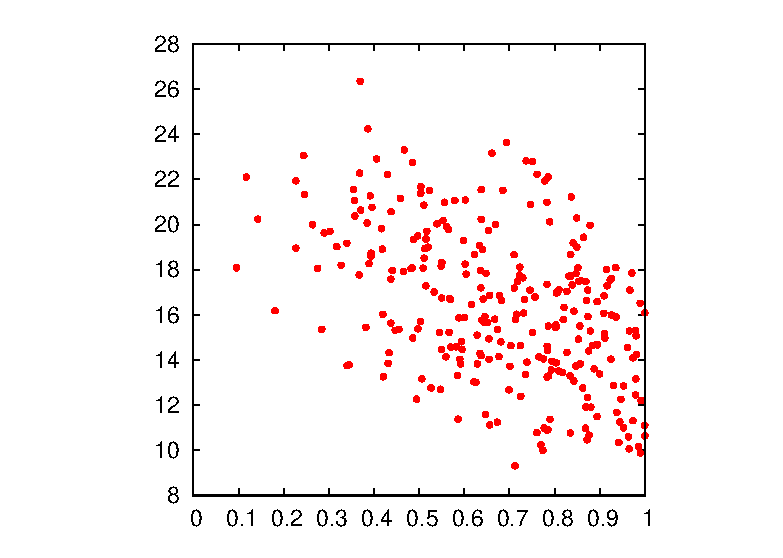
\includegraphics[width=0.4\textwidth]{./img/msms/corr-test.eps}}
\subfigure[Learn db]{
\resizebox{0.45\textwidth}{!}{\sffamily\input{./img/msms/graph-learn-fvalue-s}}}
\subfigure[Test db]{
\resizebox{0.45\textwidth}{!}{\sffamily\input{./img/msms/graph-test-fvalue-s}}}\\
\caption{\label{fig:corr}
Correlation of the system entropy $S$ and the model correctness measure
$F$-value, at temperature $T=1$. The
precursor mass is calculated from the assigned sequence.
% The correlation of those values let the user, which ignore the precursor
% sequence, to infer, from the calculated value of the system entropy, the
% expected quality of the prediction from the known distribution. 
(a) Data from 1000
random spectra with $Q=2$ from the learning database (correlation coefficient $r=-0.624$). (b) Data from
the test database ($r=-0.598$).}
\end{figure}

Despite these limitations, important information on the quality of the prediction can be extracted from the data of Figure \ref{fig:p_nu_profile}. For instance, we can select $F_0=0.8$ as a threshold for ``good'' predictions, and see how the spectra with entropy below (or above) a given threshold are classified according to this criterion.
% To this end, 
% we introduce a confidence threshold $S_0$ on the entropy of the
% prediction. Here a spectrum, whose
% interpretation shows an entropy below this threshold, can be accepted as highly
% reliable.
Table \ref{tab:corr} reports the fraction of the predictions with an entropy below a threshold $S_0$ or above $S_1$ that have $F \ge F_0$, along with the number $n$ of spectra in the dataset that fulfil the condition on the entropy.
We see, for instance, that if we set $S_0=10$ and consider the $n=$200 spectra (out of a total of 1000) that satisfy the condition $S \leq S_0$,  more than 75\% of them  present an $F$-value higher than 0.8.
In a similar way we can also introduce a second threshold, $S_1=14$, above which
the population of well-interpreted spectra is very low (less than 3\%).

\begin{table}
\begin{center}
\begin{tabular}{ccc|ccc}
\hline \hline
$S_0$ & frac & n &$S_1$ & frac& n \\
\hline
6  & 1     & 1   & 6  & 0.284  &999 \\
7  & 0.810 & 21  & 7  & 0.274  &979 \\
8  & 0.825 & 57  & 8  & 0.252  &943 \\
9  & 0.818 & 121 & 9  & 0.212  &879 \\
10 & 0.755 & 200 & 10 & 0.168  &800 \\
11 & 0.663 & 303 & 11 & 0.121  &697 \\
12 & 0.598 & 408 & 12 & 0.069  &592 \\
13 & 0.519 & 507 & 13 & 0.045  &493 \\
14 & 0.443 & 618 & 14 & 0.029  &382 \\
15 & 0.391 & 723 & 15 & 0.0072 &277   \\
16 & 0.350 & 815 & 16 & 0      &185  \\
17 & 0.327 & 872 & 17 & 0      &128  \\
18 & 0.314 & 907 & 18 & 0      &93  \\
19 & 0.306 & 932 & 19 & 0      &68  \\
20 & 0.301 & 946 & 20 & 0      &54  \\
\hline \hline
\end{tabular}
\end{center}
\caption{\label{tab:corr}
Fraction of spectra with $S<S_0$ (second column) or $S>S1$ (fifth column) with $F$-value above 0.8. 
The data refer to 1000 random spectra with charge 2, extracted from the learning dataset; column 3 and 6 report how many spectra fulfill the condition specified by the entropy threshold. 
}
\end{table}

The above results are not yet sufficient to provide the user with a definite knowledge of the value of the prediction, but are indeed a first step towards the definition of an intrinsic quality indicator of the peptide identification, a feature that is missing in other 
 \emph{de novo} sequencing approach. Future development will aim at improving the energy function, so to have a less disperse distribution, and shifted towards higher values of the $F-$value, as well as at characterizing the  probability distribution of the $F$-value versus the entropy, in order to produce reliable confidence intervals to detect false positives and false negatives.






%We define a symbol entropy $\mathcal S$ as:
%\begin{equation}
%\mathcal S = -\sum_\nu \Bigg[\Big(\sum_i p_\nu(s_i)\Big)
%\log \Big(\sum_i p_\nu(s_i)\Big)\Bigg]
%\end{equation}
%that measure the capacity of the system to adapt to the energy landscape. At
%temperature $T=1$ we find that the correlation with the $F'$-value is of about
%-0.675717. It is handy to the purpose of predicting a peptide sequence without
%the knowledge of the actual real sequence.
%{\bf qui bisogna fare un paragrafo meglio con i dati che stiamo aspettando}






